\section*{2}

Dado el conjunto $M \subset \R^2$ definido por
\begin{equation*}
    M = \{(x_1 , x_2 ) \in \R^2 : x_1 \leq x_2 , x_2 \leq -x_1^2 + 2\},
\end{equation*}
se considera la función de $\R^2$ en $\R$ que a cada punto de $\R^2$ le asocia su distancia al origen,
y se trata de obtener los puntos de M cuya distancia al origen es máxima y mínima.
Formule el problema de optimización, indicando la función objetivo y el conjunto factible y resuélvalo gráficamente utilizando curvas de nivel.

\noindent\rule{10cm}{0.4pt}

Para obtener los puntos de $M$ cuya distancia al origen es minima planteamos el siguiente problema de optimización,
\begin{equation} \label{ex1_min_implicit}
\begin{aligned}
    \text{Minimizar }   & x_1^2 + x_2^2 \\
    \text{sujeto a }    & (x_1, x_2) \in M,
\end{aligned}
\end{equation}
donde la funcion objetivo es $x_1^2 + x_2^2$ y el conjunto factible es $M$.

Podemos hacer que las restricciones del problema \ref{ex1_min_implicit} sean explicitas,
\begin{equation} \label{ex1_min_explicit}
\begin{aligned}
    \text{Minimizar }   & x_1^2 + x_2^2 \\
    \text{sujeto a }    & x_1 \leq x_2, \\
                        & x_2 \leq -x_1^2 + 2.
\end{aligned}
\end{equation}

Resolviendo el problema \ref{ex1_min_explicit} gráficamente usando \textit{Python} y \textit{matplotlib}
vemos que el problema tiene un único mínimo localizado en el origen, como vemos en al figura \ref{ex1_min}.

\begin{figure}[h]
\centering
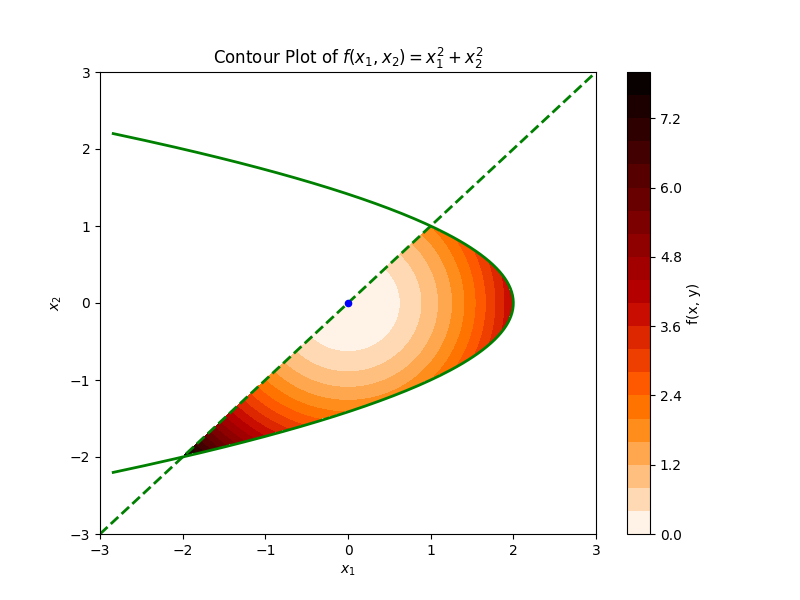
\includegraphics[scale=0.6]{ex1_min.png}
\caption{Solución gráfica para el problema de minimizar.}
\label{ex1_min}
\end{figure}

Para encontrar el punto con distancia maxima al origen planteamos el siguiente problema de maximización.
\begin{equation} \label{ex1_max_explicit}
\begin{aligned}
    \text{Maximizar }   & x_1^2 + x_2^2 \\
    \text{sujeto a }    & x_1 \leq x_2, \\
                        & x_2 \leq -x_1^2 + 2.
\end{aligned}
\end{equation}

Resolviendo el problema \ref{ex1_max_explicit} gráficamente,
obteniendo la figura \ref{ex1_max} 
y vemos que el problema tiene un único mínimo localizado en el el punto $(-2,-2)$.

\begin{figure}[h]
\centering
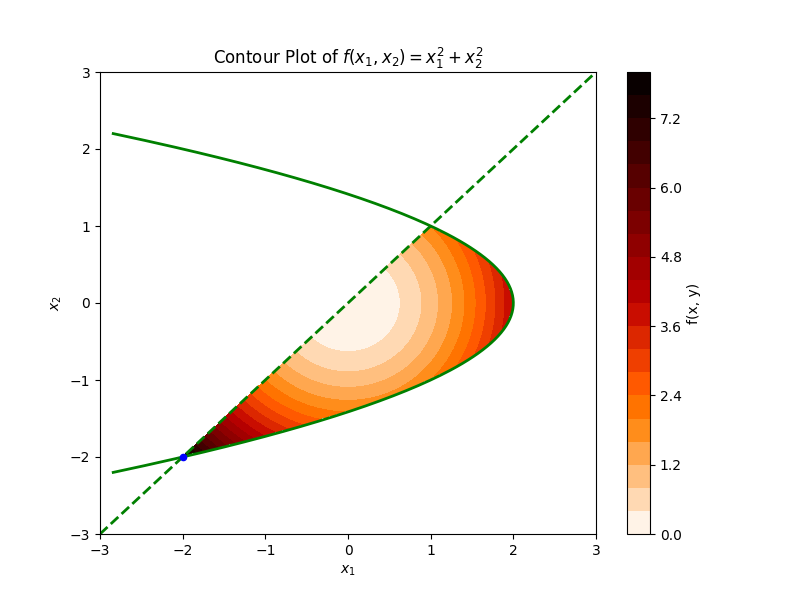
\includegraphics[scale=0.6]{ex1_max.png}
\caption{Solución gráfica para el problema de minimizar.}
\label{ex1_max}
\end{figure}
